\chapter{Exploiting classical nucleation theory for reverse self-assembly}
\label{chap:pixel}

\section{Introduction}

Not only is understanding, controlling and predicting the phenomenological behavior of particle self-assembly one of the great mathematical challenges for the twenty-first century, but its applications in materials science and engineering hold promise for the development of materials with novel electronic, mechanical, and optical properties.
Although most of the work performed in this field is historically rooted in the self-assembly of small molecules, the last decade has witnessed extraordinary advances in particle synthesis at the mesoscale~\cite{DeVries,Schnablegger,Hong,Weller,Hobbie}, making possible the production of  building blocks  with complex chemical and geometrical properties with an unprecedented degree of precision.
Unfortunately, a coherent theoretical framework around the problem of self-assembly is still missing, and numerical simulations have taken the lead in exploring the wealth of new phenomenological behavior arising from the collective behavior of nonisotropic components.

Most  numerical studies on self-assembly of nanoparticles performed so far have adopted the patchy sphere model~\cite{Kern}.
In this model, the isotropicity of a particle is broken by placing on its surface regions (patches) with different physical properties; for example, hydrophobic chemical groups or single-stranded DNA chains.
Theoretically, these regions are incorporated into the interparticle potential by a simple angular dependence which favors or disfavors the alignment of such patches -- in practice, the patchy sphere model can be thought of as a generalization of the amphiphilic model used in Chapter~\ref{chap:janus} to include more than one hydrophilic region.

Although self-assembly of several simple  structures has been achieved with patchy models (references \cite{glotzer4,Liu,cacciuto} are just a few examples of the large body of work published on the subject; for a recent review see references~\cite{sciortino1,sciortino2}), a general modeling approach to the problem is missing.
Shape and position of the interaction sites is either guessed using physical arguments, or inspired by known molecules or protein structures aggregating into a similar target crystal.

There are three notable exceptions.  \citeauthor{torquato}~\cite{torquato} proposed an inverse optimization technique.
In this technique, an isotropic (two-dimensional) interaction potential is sought by choosing a family of functions $\phi(r; a_0, a_1, ..., a_n)$, parametrized by the $a_i$s.
Reverse self-assembly is achieved either by choosing an objective function such that the energetic stability of the target crystal is maximized with respect to competitor lattices (``zero-temperature'') or by running finite temperature simulations and minimizing the Lindemann parameter $\Theta_2$.
The success of this method relies on a suitable choice of $\phi$.
Furthermore, this technique is specific to nondirectional interactions, and while examples are provided of such potentials yielding complex and surprising self-assembled structures, these potentials are sufficiently complicated that they are not achievable experimentally.

Additionally, \citeauthor{glotzer7} have developed so-called ``bottom-up building block assembly,'' or BUBBA~\cite{glotzer7,glotzer8}.
This method requires the construction of the entire self-assembly pathway up to the target structure, and thus is primarily applicable to simple cases in which particles interact in a very defined way, such as the so-called tetrominoes on a grid, for which it has been demonstrated.
Furthermore, BUBBA requires construction of the partition function of the system, starting from individual particles; while the authors have demonstrated in~\cite{glotzer8} a method for choosing the most relevant terms of the partition function and thus reducing the computational complexity, the degree of allowable complexity is currently very low.

Finally, \citeauthor{brenner}~\cite{brenner} have described a method by which the yields of specific, finite clusters (for example, a tetrahedral [$T_d$] cluster) can be enhanced by using nonidentical spheres.
In the case of a $T_d$ cluster, eight different particle types are used, and an $8 \times 8$ matrix of particle interaction energies is constructed. 
Given this matrix, the total energy of all possible configurations of eight-particle clusters given those interparticle interactions are calculated (totalling $504,000$ configurations for eight-particle clusters).
The optimal set of particle interactions is the one in which the desired cluster is the ground state and the standard deviation $\sigma$ is less than some critical value (set by the parameters of the system).
While this method is useful for designing interactions for yielding finite structures, it has a similar limitation to the BUBBA method: it requires the enumeration and energy calculation of all possible competing structures, which is unfeasible for even moderately complex or large structures.

The development of an efficient numerical procedure to design interactions between nanoparticles that targets specific crystal structures via the process of self-assembly would therefore be a result of great importance. 

As discussed in Chapter~\ref{chap:janus}, while the generic features of particle aggregation can be described in terms of simple thermodynamic arguments, the details of the process can be very complex and multi-faceted.
In fact, a full theoretical description of this problem must incorporate critical kinetic effects which are not captured by classical thermodynamics, and which have dramatic macroscopic consequences~\cite{chandler, cacciuto,whitelam}.
 
It is now understood that for self-assembly to take place, a very delicate balance between entropic and energetic contributions, coupled to a precise geometric character of the components, must be satisfied. 
In general, self-assembly of nanocomponents is not to be expected unless a careful design of the building blocks has been performed beforehand~\cite{chandler, cacciuto}.

\begin{figure}
	\begin{center}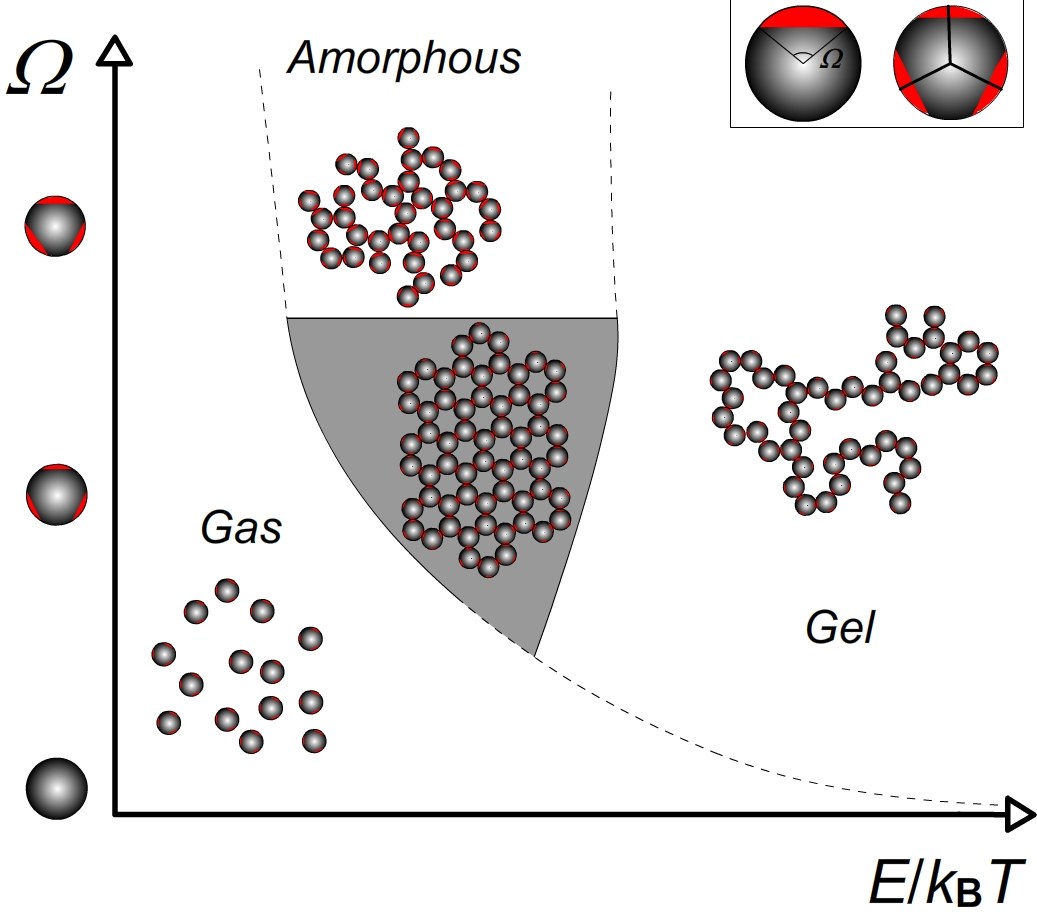
\includegraphics[width=0.6\textwidth]{pixel/generic.png}\end{center}
	\caption[Generic self-assembly diagram for patchy spherical particles]{Illustration of a generic self-assembly diagram for patchy spherical particles
	expected to aggregate into a honeycomb lattice. $E$ is the interparticle attraction strength and
	$\Omega$ is the angular size of the patches.}\label{patches}
\end{figure}

Figure~\ref{patches} illustrates the problem for a simple model: spherical particles with attractive patches oriented to form a two dimensional honeycomb lattice.
When the angular size $\Omega$ of each patch is too large, the interaction is not specific enough to select the desired crystal, resulting in amorphous structures originating from the competition of multiple fitting geometries.
If $\Omega$ is too small (too specific), the probability that two particles in close proximity are properly aligned to interact becomes negligible, and the system is found in a gas phase unless a very large interparticle energy $E$ is provided, which in turn drives the system into a gel  phase.

Analogous arguments can be made for the overall strength of the interaction that, for a reasonable patch size, should be neither too strong nor too weak.
The net result is that self-assembly is a very elusive process that requires a careful design and fine tuning of the interparticle interactions, and typically the target region in the interaction space in quite narrow.
 
Our interest is in the problem of ``reverse self-assembly,'' in analogy to the problem of ``reverse protein folding'' in which protein sequences are designed to yield a desired ground-state folded structure~\cite{Yue, Deutsch}.
The problem can be formulated as follows: given an arbitrary final structure, is there an efficient method by which interparticle interactions may be designed so that the particles spontaneously self-assemble into the given structure?

In this chapter we use simple physical arguments to develop a numerical procedure capable of sampling the space of interactions, in terms of both patch geometry and binding energy, to generate nanoparticle interactions leading to self-assembly of desired crystal structures.
Without loss of generality, we limit our discussion to spherical particles interacting via anisotropic short-range attractive pair potentials mimicking the hydrophobic interactions, such as those used in Chapter~\ref{chap:janus}, driving self-assembly of Janus particles~\cite{Hong2, cacciuto}.    
 
Classical nucleation theory provides a simple framework within which to think about crystal formation.
Recall from Section~\ref{sec:CNT} that the free energy $\Delta G$ associated with crystal nucleation is given by
\begin{equation}\Delta G \simeq \frac{4}{3} \pi r^3 \rho \Delta \mu + 4 \pi r^2 \gamma \,.\end{equation}
This leads to the critical nucleus size, $n^* = \frac{32 \pi}{3 \rho}\left(\frac{\gamma}{\left|\Delta \mu\right|}\right)^3$, above which the crystal will grow until the phase transition is completed and below which the crystal will vanish.
Thus, we have a curve as illustrated in Figure~\ref{fig:CNT}, where the maximum in $\Delta G$ (and thus the point where $\frac{d\Delta G}{d n} = 0$) occurs at that point $n^*$.

We argue that a successful strategy for crystal design should take into account the physical properties of the parent fluid phase, and our working hypothesis is that the free energy of crystal nucleation can be exploited to design interactions to target arbitrary crystal structures.  
The main idea is to force a crystal nucleus of desired symmetry to be in contact with its own fluid and use a numerical procedure to select for those interactions between the particles that minimize the free energy cost required to hold that nucleus in place.
Our scheme consists of two parts: 1) we determine  the optimal shape of the hydrophobic regions ($\Omega$) satisfying the condition stated above, and 2) given $\Omega$, we find  the interaction strength ($E$) for which the system is likely to nucleate into the target (defect-free) crystal phase.  

\section{Sampling the interaction shape $\Omega$}

Consider a system of $N$ identical particles with a given interparticle potential $U(\Omega_i,r)$, where $\Omega_i$ is the interaction shape (which will be kept to a very general definition at this point) and $r$ is the interparticle distance, set in a volume $V$.
Define an order parameter $q$ capable of detecting the symmetry of the desired crystal phase (an example of such an order parameter for fcc crystals is described in Section~\ref{sec:orderparamdesc}; other order parameters are described below).

Grow from the fluid and equilibrate a crystalline nucleus of size $n_0$ using a standard biased Monte Carlo method targeting the size of the largest crystalline cluster in the system, $n$, via a potential~\cite{tenwolde2} 
\begin{equation}
	V_B(n)=\frac{\kappa}{2} (n-n_0)^2 \,.
\end{equation}
Set the binding energy among the particles to a sufficiently small value to ensure that the nucleus melts once the bias is removed, and compute from a full, but short, simulation in the presence of the bias the average crystal size $\bar n(\Omega_i)$.

Now define a (fictitious) design potential 
\begin{equation}
	V_D[\bar n(\Omega_i)]=-\alpha \bar n(\Omega_i) \,,
\end{equation}
where $\alpha$ is a numerical constant. 
At this point the idea is to sample over the space of interactions using $V_D$ as a driving force.
Specifically, we generate an alternative (trial) shape for the interaction between any two particles in the system $\Omega_j=\Omega_i+\Delta\Omega$ and repeat the previous steps to obtain a new estimate for $V_D[\bar n(\Omega_j)]$.
$\Omega_j$ is accepted or rejected based on a standard Metropolis criterion, thus ensuring that the $\Omega$ will be driven towards values that maximize the size $\bar n$.
Because the interaction energy has been set in such a way that the thermodynamic force on the system is in the direction of melting the crystal, maximization of $\bar n$ is equivalent to minimization of the load requested of the bias to hold the crystal in place.
 
\section{Sampling the interaction strength $E$}

Unfortunately, our method does not allow easy measurement of the height of the nucleation barrier given an interaction strength $E$.
This is mostly because the surface tension between the crystal and the fluid phase is unknown.
Nevertheless, we have direct access to the slope of the free energy barrier.

Therefore, although one cannot design the system to comply with a specific nucleation rate $\nu$, by modulating $E$ one can design the size of the critical nucleus $n^*$. 
A critical nucleus that is too small will result in the almost instantaneous nucleation of several crystallites that will form defects and grain boundaries as they meet while growing.
The opposite scenario will lead to absence of crystallization within the experimental time frame.
For the systems we have examined, we find that $15 \lesssim n^* \lesssim 30$ results in nucleation events that are quick, yet sufficiently rare to prevent formation of multiple crystals.
The choice of $n^*$ may require a few iterations depending on the details and the size of the system.

The strategy behind the design of the critical nucleus size is analogous to that described in the previous case, except that the design potential in this case has a harmonic functional form defined as
\begin{equation}
	V_D[\bar n(E_i)]=\alpha (\bar n(E_i)-n^*)^2 \,,
\end{equation}
and we sample over the interaction strength $E$.
Minimizing $V_D$ implies that the system will be driven towards that value of $E$ (defined as $E^*$) for which the nucleus has the same probability of growing or shrinking, yielding, on average, $\bar n(E_i) = n^*$.
This condition guarantees that the system is at the top of the nucleation free energy barrier, since to either side of the critical point there is a definite direction in which the value of $\bar n$ will move.
Thus, $n^*$ has indeed become the critical nucleus by definition.

Note that in principle, the interaction geometry could have an arbitrary number of parameters that could all be optimized simultaneously; however, it is crucial that the optimization of the geometry precedes the optimization of the strength of the potential.
The algorithm for the optimization of interaction geometry relies upon the nucleus being precritical; otherwise, it will be completely ineffective.

\section{Numerical tests}

As a proof of concept for our method we consider the design of two distinct crystal structures for which we can guess the solution in the interaction space and know how to define an order parameter $q$: a simple cubic crystal (SC) and a two dimensional sheet with square symmetry embedded in a three dimensional environment (2SQ).

For both systems we adopt the Kern-Frenkel model~\cite{Kern}. 
Particles are described as hard spheres of diameter $\sigma$ interacting via a short-range attractive interaction that is turned on whenever hydrophobic regions (the patches) on different particles face each other.
For each  pair of particles $i$ and $j$ with patch indices $\alpha$ and $\beta$, the interaction is defined as 
	\begin{equation}
		\label{eq1}
		u(\mathbf{r}_{ij})=u_{\rm SW}(r_{ij}) \sum_{\alpha,\beta}f^{\alpha\beta}(\Theta_{ij}) \,,
	\end{equation}
where $ u_{\rm SW}(r_{ij})$ is a standard attractive isotropic square well potential of depth $\varepsilon$ and range $1.15\sigma$, and $f^{\alpha\beta}(\Theta_{ij})$ depends on the particles' mutual orientations and is defined as
	\begin{equation}
		\label{eq2}
		f^{\alpha\beta}(\Theta_{ij})= \left\{
		\begin{array}{ll}
			1 &\mbox{if \, }\left\{
			\begin{array}{lll} \mbox{ \,\,\,\,\,\,\, \,\,\,${\bf r}_{ij}\cdot{\bf e}_{\alpha}>\cos \theta$ } & \begin{array}{l}\end{array} &\\ 
    			\mbox{ and ${\bf r}_{ji}\cdot{\bf e}_{\beta}>\cos\theta$ } & \begin{array}{l} \end{array}
            \end{array} \right.\\
		0 & \mbox{otherwise}
		\end{array} \right. \,.
	\end{equation}

Here $\theta$ is the angular size of the hydrophobic regions (selected to be all identical in size and circular in shape), ${\bf r}_{ij}$ is the unit vector along the direction of the interparticle separation, and ${\bf e}_{\alpha}$ is the unit vector connecting the center of a particle to the center of the patch $\alpha$ on its surface.
 
In these simple systems $\theta$ and $\varepsilon$ are the design parameters we need to tune for self-assembly to take place.
All simulations are performed in the $NVT$ ensemble using a minimum of 256 particles in a box with periodic boundary conditions.
A good order parameter to detect SC crystals is the standard local bond order based on spherical harmonics, $\bar{q}_4$; that is, $q_l$ from Section~\ref{sec:orderparamdesc}, where $l = 4$ for the detection of crystals of four-fold symmetry.
A particle $i$ is tagged as crystalline if $\bar{q}_4$ is greater than a chosen cutoff, $q_{\rm {cut}}$ -- the sensitivity of the technique to the choice of order parameter is discussed in Section~\ref{sec:limitations}.
 
For the 2SQ case we used $\bar{q}_4$ with the added constraint that a particle must have interactions with no more than four neighbors in order to be considered ``crystalline.'' The location of the patches -- or, in particular, the absence of patches on the ``poles'' of the particles -- automatically prevents the formation of SC crystals in this case. The insets in Figure~\ref{fig:force} sketch the patch positions over the particles.

\begin{figure*}
	\begin{center}\subfloat[]{
		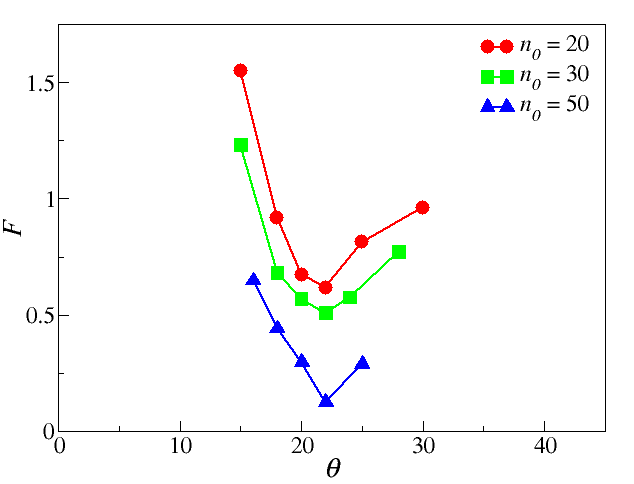
\includegraphics[width=0.6\textwidth]{pixel/SCxtalsize.png}
		\put(-80,25){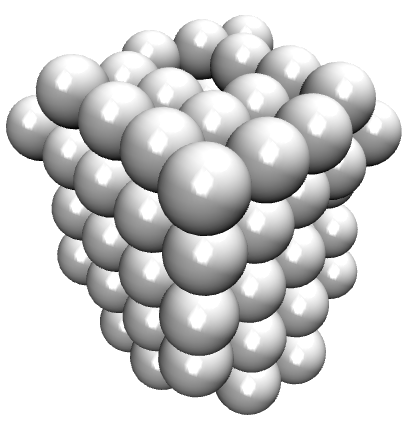
\includegraphics[width=63px]{pixel/SCimage.png}}
		\put(-230,35){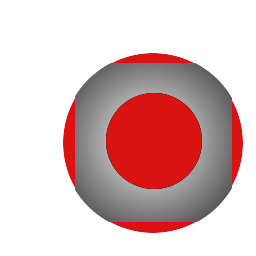
\includegraphics[width=45px]{pixel/6patch.png}}
		\label{force:SC}
	}

	\subfloat[]{
		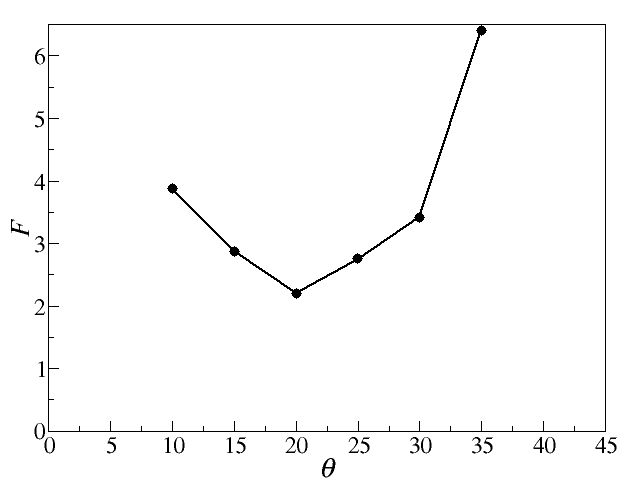
\includegraphics[width=0.6\textwidth]{pixel/2SQforce.png}
		\put(-92,25){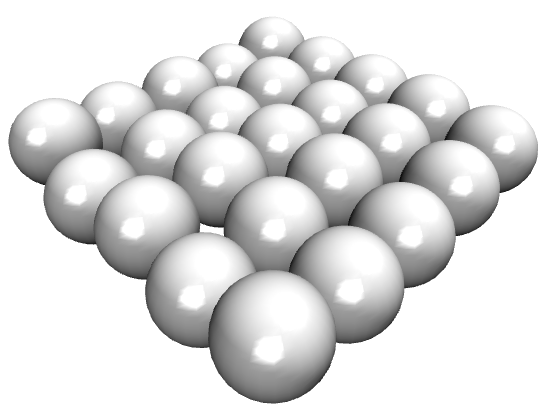
\includegraphics[width=75px]{pixel/2SQimage.png}}
		\put(-230,35){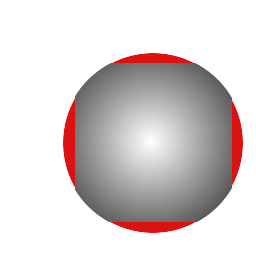
\includegraphics[width=45px]{pixel/4patch.png}}
		\label{force:2SQ}
	}\end{center}
	\caption[Force vs. $\theta$ for square cubic and 2D square crystals]{Force vs. $\theta$ for \subref{force:SC} SC and \subref{force:2SQ} 2SQ crystals.  The insets show snapshots of the target crystals, and  sketches of the locations of the patches in our particle model. In
\subref{force:SC}, the different lines represent data obtained by imposing different nucleus sizes $n_0$ as indicated
in the legend.}\label{fig:force}
\end{figure*}

Figures~\ref{force:SC} and~\ref{force:2SQ} illustrate how the force $F(\theta)=-\kappa (n-n_0)$ required to hold a nucleus of $n_0$ particles immersed in its fluid phase depends on the size of the circular regions $\theta$ for the SC  and the 2SQ crystals, respectively.

The corresponding simulations were performed at densities of $\rho_{SC} = 0.1$ and $\rho_{2SQ} = 0.01$, binding strength $\varepsilon_{SC}=3.5k_{\rm B}T$ and $\varepsilon_{2SQ} = 5.75k_{\rm B}T$, and a harmonic bias potential of spring constant \textcolor{black}{$k_{SC} \simeq 0.2k_{\rm B}T$} and \textcolor{black}{$k_{2SQ} = 0.4 k_{\rm B}T$}.
Clearly, $F(\theta)$ is a sufficiently sensitive parameter to discriminate among the different angular sizes,  and presents in both cases a distinct optimal value; $\theta^*_{SC}\simeq 22^{\circ}$ and $\theta^*_{2SQ}\simeq 20^{\circ}$.
Figure~\ref{force:SC} also shows that the optimal value is fairly independent of  the particular average size 
$n_0$ of the nucleus held in contact with the fluid.
Figure~\ref{trajectory} shows how the location of $\theta^*$ and $\varepsilon^*$ can be obtained automatically by using the Monte Carlo scheme in the space of interactions, using $n^* = 20$.

\begin{figure*}
	\begin{center}\subfloat[]{
		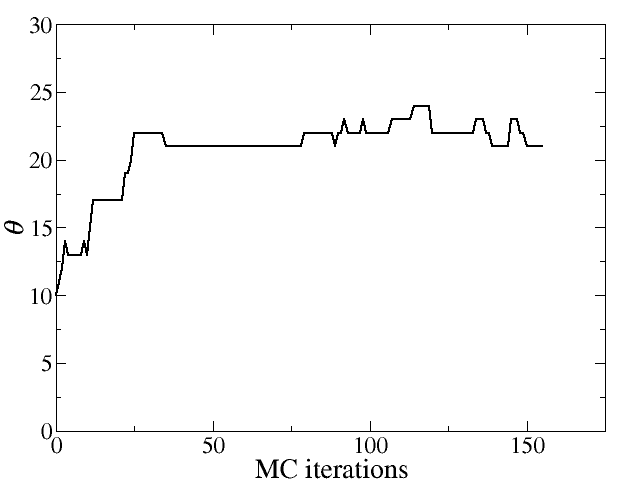
\includegraphics[width=0.6\textwidth]{pixel/TJtheta.png}
	}

	\subfloat[]{
		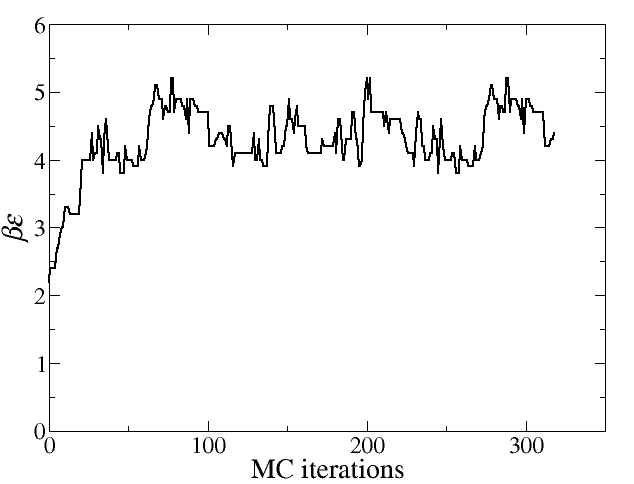
\includegraphics[width=0.6\textwidth]{pixel/TJenergy.png}
	} \end{center}
	\caption[MC trajectories in interaction space for the design of simple cubic crystals]{Monte Carlo trajectories in the space of interactions for the design of the simple cubic crystal. In (a) the shape of the patches defined by the solid angle $\theta$ is allowed to fluctuate while keeping the strength of the interaction $\varepsilon$ constant. In (b) $\varepsilon$ fluctuates while keeping $\theta$ constant and at the optimal value found in (a).}	\label{trajectory} 
\end{figure*}

It should be stressed that the minimization of $V_D[\bar n(\Omega_i)]$ can be achieved using any minimization algorithm; nevertheless, we find that the Monte Carlo scheme allows us to use shorter simulations, for each trial $\theta_i$, than would be necessary for other direct minimization schemes.
The reason is related to the precision of the estimate of $\bar n$ for relatively short trajectories, which could be 
over- or underestimated.
This could lead to fictitious local minima, which could trap a direct minimization scheme, but are easily overcome with a standard Monte Carlo method.
 
\begin{figure*}
	\begin{center}\subfloat[]{
		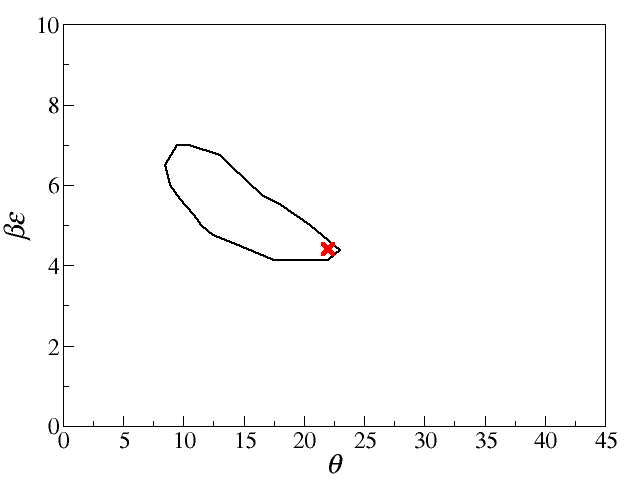
\includegraphics[width=0.6\textwidth]{pixel/SC.png}
		\label{phase:SC}
	}

	\subfloat[]{
		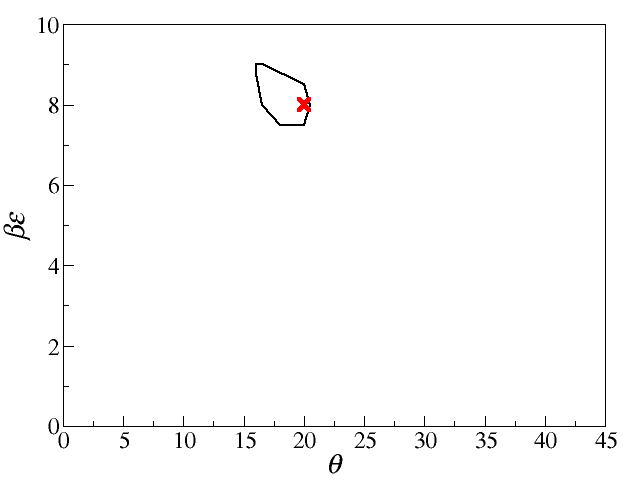
\includegraphics[width=0.6\textwidth]{pixel/2SQ.png}
		\label{phase:2SQ}
	}\end{center}
	\caption[Phase diagrams for simple cubic and 2D square crystals]{Phase diagrams for \subref{phase:SC} SC and \subref{phase:2SQ} 2SQ crystals.  Lines show the border around the phase region in which particle form the desired crystal; the points marked by an `\textcolor{red}{X}' are the $(\theta, \beta\varepsilon)$ combinations found to be optimal by our method.}\label{phase}
\end{figure*}

In order to check our method, $\varepsilon-\theta$ phase diagrams were constructed using the traditional, ``forward'' method of trial-and-error\textcolor{black}{, running Monte Carlo simulations for $10^7$ steps and determining whether crystallization into the desired structure occurred using the order parameters discussed above as well as direct inspection}.
As shown in Figure~\ref{phase}, the parameters detected by our methods are within the crystallization regions for the two target crystals.
Unsurprisingly, the result falls roughly to the high-$\theta$, low-$\varepsilon$ edge of the crystallization region; recall that $\theta$ was selected using a value of $\varepsilon$ too low for crystallization, which would be expected to result in a larger $\theta$ (note the roughly inverse $\varepsilon-\theta$ relationship in Figure~\ref{phase}); $\varepsilon$ was then selected using the $\theta$ found in the first step.

\section{Limitations}\label{sec:limitations}
It is important to discuss the limitations of the method.
First of all, in its actual formulation, our method only works for systems  that will self-assemble into an infinitely large aggregate via the process of nucleation.
It is not obvious how to generalize it to include self-assembly into finite size aggregates such as, for instance, viral capsids, although this is obviously a regime in which such design would be very desirable.

The second limitation is that although the method provides a solution to the reverse self-assembly problem, there is no guarantee that the solution is the optimal one.
This is because our method forces the  nucleation process to follow the classical route, i.e. the forming nucleus has the same structure as the  target crystal; however, there are several examples~\cite{tenwolde,cacciuto22,whitelam,kumar} where the nucleation barrier may be lowered by following a more complex dynamical pathway that may include metastable states having different symmetry than that of the target crystal -- Chapter~\ref{chap:janus} clearly illustrates this principle for asymmetric Janus particles.
For instance, it is possible to imagine that the formation of the SC crystal could benefit from an additional weak, non-specific, isotropic interaction, on top of that provided by the patches, that may initially lead the system into a high-density metastable fluid phase from which nucleation into the final structure may proceed at a faster rate than that predicted otherwise (analogous to the dense fluid aggregates that formed in Chapter~\ref{chap:janus} from which fcc crystals nucleated).

Finally, it is crucial to develop a good order parameter $q$ to describe the desired crystal structure.   
Figure~\ref{orderparameter} illustrates how an inefficient order parameter may lead to fictitious minimization in the space of interactions while designing the 2SQ crystal.
The different lines in the $F$ vs. $\theta$ diagram represent different values of $q_{\rm cut}$ (defining how restrictive the order parameter is) from $0.8$ to $0.99$.

We find that a cutoff in the order parameter of at least $0.97$ is required to adequately distinguish between the square and hexagonal symmetries for large values of $\theta$.
The curves related to the less restrictive order parameters would in fact misleadingly indicate a flatter bottom of the curve, while in reality we find that any angle larger than $\sim25^{\circ}$ will lead to nucleation into a two-dimensional crystal with hexagonal symmetry. 
Adding an energy penalty to  prevent arrangements compatible with the competing six-fold symmetry (apart from imposing a limit to the number of neighbors), using an order parameter such as the familiar $\bar q_6$, may also be considered as a means of improving the design procedure.

\begin{figure}
\begin{center}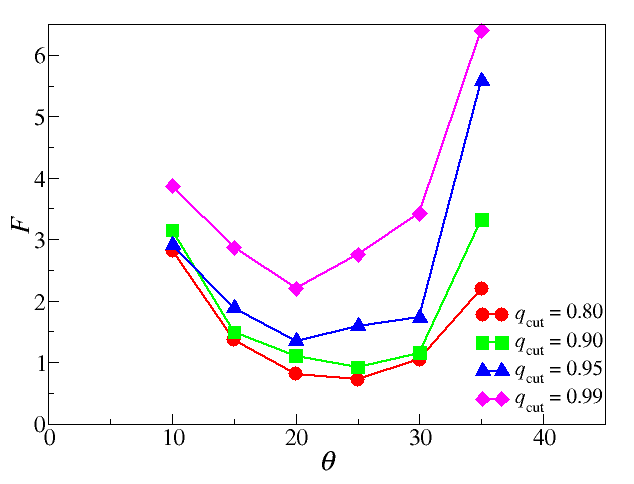
\includegraphics[width=.6\textwidth]{pixel/2SQorderparameter.png}\end{center}
\caption[F vs. $\theta$ for different values of the order parameter $q_{\rm cut}$]{$F$ vs. $\theta$ diagrams.  The dependence of the method on the order parameter used.  Different curves correspond to different values of the  cutoff $q_{\rm cut}$.} \label{orderparameter}	 
\end{figure}

{\section{Beyond the Kern-Frenkel model}
Here we propose a more general model to describe interparticle interactions that we name the {\it Adaptive Pixel Model}.
The idea stems from the need to devise a  way of sampling over different geometric patterns (beyond circular) in search of those which can efficiently hold the single components into a desired target structure.
The first step is the discretization of the surface of the particle.

For spherical building blocks, we cover the surface of each particle with a large number, $N_p$, of regularly-spaced interaction sites (pixels) as illustrated in Figure~\ref{pixels}.
A good arrangement of the pixels can be obtained by using the spherical triangulation provided by an $(n,m)$ delta-icosahedron~\cite{geom}, and $N_p$ is selected depending on the complexity of the target structure.
Euler's theorem imposes the following constraint on  $N_p$: $N_p=10(n^2+nm+m^2)+2$~\cite{geom}, where $n$ and $m$  indicate that one has to move $n$ pixels  along the row of neighboring bonds on the sphere, and then after a turn of $120^{\rm o}$, move for $m$ extra pixels. 
 
In the simplest version of the model, to each pixel $k$ on a particle $i$ is assigned a variable $s_i^k$ which has a binary character, $s_i^k\in\{1,0\}$ depending on whether that  interaction site is switched {\it on} or {\it off}.
Whenever two particles $i$ and $j$ are within a given distance of each other, the axis between them, ${\bf{r}}_{ij}$, is calculated.
If the nearest digit to the point where ${\bf{r}}_{ij}$ crosses the surface of each particle is {\it on}, then the particles feel an overall short-range attractive interaction.

Pixels on the same particle do not interact with each other.
The interaction pair potential between any two particles, $i$ and $j$, of diameter $\sigma$, set at a distance $r_{ij}$ from each other, then takes the form
	\begin{equation}
		V(r_{ij}) = V_{\rm HS} + \begin{cases} 	-s_i^ks_j^l\varepsilon		&	\textrm{if } |r_{ij}| \leq r_0 \\
											0 							&	\textrm{otherwise}\end{cases} \,,
		\label{interaction}
	\end{equation}
where $s_i^k$ and $s_j^l$ are the binary variables corresponding to the digits intersected by $r_{ij}$ on particles $i$ and $j$, respectively, as described above.
Excluded volume between the particles is enforced via a standard hard-sphere potential, $V_{\rm HS}$. 
	\begin{figure}
		\begin{center}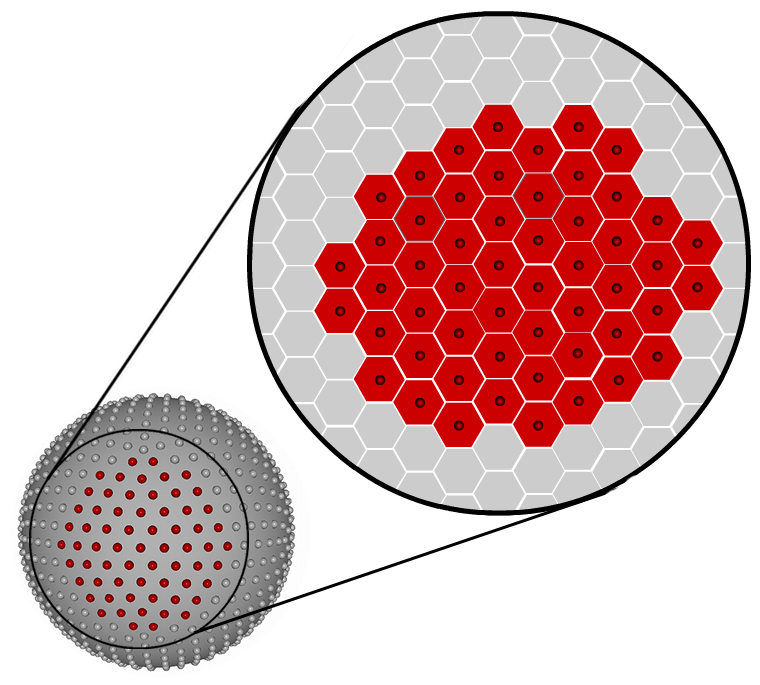
\includegraphics[width=0.6\textwidth]{pixel/digits.png}\end{center}
		\caption[Illustration of the structure of the {\it Adaptive Pixel Model}]{Illustration of the structure of the {\it Adaptive Pixel  Model}. {\it On} pixels are depicted in red while {\it off} pixels are in gray. The magnification in the top image shows the Voronoi tessellation around the pixels (computed as described in the text). The effective geometry of the active sites in this representation is a hexagon. }
		\label{pixels}
	\end{figure} 

The main advantage of this setup is that once particles are held into place at given positions, the geometry of the interacting regions emerges as a result of a simple Monte Carlo simulation on $s_i^k$ which samples different states according to Equation~\ref{interaction}.
Such a simulation is analogous to the simulation of a simple Ising model, but in which the energy depends not on the neighboring pixels on the same particle but on pixels on neighboring particles.

Crucial to the efficiency of the model is the independence of the interaction strength of the total area of the attracting region.
This condition, also assumed in the Kern-Frenkel model, is appropriate when considering interactions that have a range of action that is small compared to the colloidal diameter (($r_0-\sigma)\lesssim 0.15\sigma$), and allows us to circumvent the overwhelming cost related to the computation of the $N_k^2$ distances between the pixels.

Furthermore, as the relative distances of on-particle pixels are frozen and only active pixels need to be tracked, it is possible to perform the
search of the nearest pixel to any point on the sphere very efficiently.
This is achieved by creating a cell list over the spherical particle surface in $\theta$ and $\phi$ (the spherical coordinates), and by associating with each cell the identity of the nearest pixel.
This is equivalent to generating a discrete Voronoi tessellation~\cite{geom} of the spherical surface based on the pixel locations (see sketch in Figure~\ref{pixels}), which needs to be performed only once at the beginning of the simulation.
Any shape for the interaction regions can be achieved by simply switching {\it on} or {\it off} pixels or groups of pixels. }

\section{Conclusions}

In this chapter we have proposed a simple two-step method for the problem of reverse self-assembly.
The idea is to exploit the curvature of the nucleation free-energy barrier to sample and select optimal interparticle interactions for self-assembly into a target structure.
Numerical simulations have been presented to test the efficacy of our method, as well as detailed discussion of its limitations and its potential. 
These simulations show that our method reduces the time to solve the problem of determining optimal interaction parameter from on the order of weeks (for trial-and-error approaches) to hours.

Finally, we proposed a new model, the {\it {Adaptive Pixel Model}}, by which almost any interaction geometry can be realized in a simple and efficient way.
It should be stressed that our method is not limited to spherical particles but can be applied to any particle shape;
in principle, particle shape could be introduced as a new parameter in the interaction space and be sampled over using the scheme proposed in this paper.

Although our method does not capture the dynamical subtleties of the crystal formation process, it does provide a very efficient way of screening over a large number of given interaction geometries that can be mapped onto the pixels.
Efficient ways of sampling the interaction space could be obtained using genetic algorithms that can be used to evolve optimal interaction patterns given a set of initial shapes. 
